\chapter{Goals and Use Cases}
\label{ch:Goals and Use Cases}

In this chapter, we discuss the intended goals of the project and list some use cases.

\section{Goals}

\paragraph{}
The goal of the project is to develop a software suite which facilitates interoperability between MANO frameworks, thereby enabling management of a network service across multi-vendor environments. To achieve this, we're dividing the software suite into 3 individual work packages (WP), which are developed in parallel initially and finally be merged. In the following sections, we discuss the individual goals of these work packages in detail.

\subsection{WP1: Service Descriptor Translator (SDT)}
\paragraph{}


\subsection{WP2: Service Descriptor Splitter (SDS)}
\paragraph{}


\subsection{WP3: MANO Scalability Support}
\paragraph{}


\subsection{Integration Of Work Packages}
\paragraph{}


\begin{figure}
	\centering
	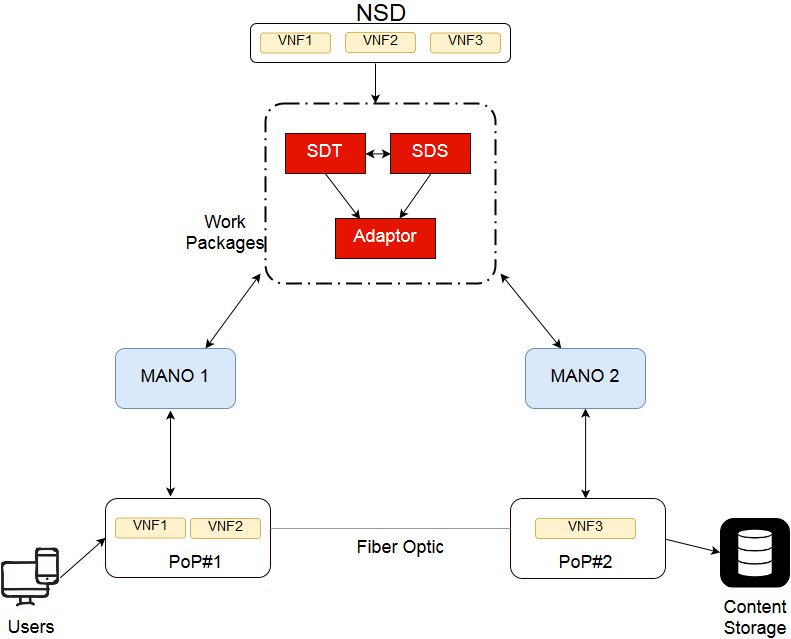
\includegraphics[width=0.7\linewidth]{figures/Structure_Updated1}
	\caption{This figure visualizes the structure of the project. }
	\label{fig:structureupdated1}
\end{figure}


\newpage
\section{Use Cases}

\subsection{Cross-MANO Framework Interaction}
\paragraph{}

The MANO frameworks used by every network service provider varies from one another. NSD translation enables the deployment of network services that is in accordance with the intended framework.

For instance : If an operator uses Sonata framework and another operator uses OSM framework, the NSD schemas for both the frameworks will be different. Using the solutions of translation and splitting, network services can be deployed and orchestrated across different MANO implementations.

\subsection{Hierarchical Orchestration}
\paragraph{}
By implementing MANO adaptor, dynamic instantiation and inter-operability between different MANO frameworks can be achieved. As a result, operators will be able to scale up and scale down the resources as and when required.

 Also, the operator will be able to handle the resources in an efficient manner. 
When there is a high demand for network service, the operator can explore options to include additional MANO instances to mitigate the traffic load on a single MANO instance. The resources can be provisioned based on the number of requests. This helps the operator in extending their profitability. 

























